\begin{figure*}
\centering
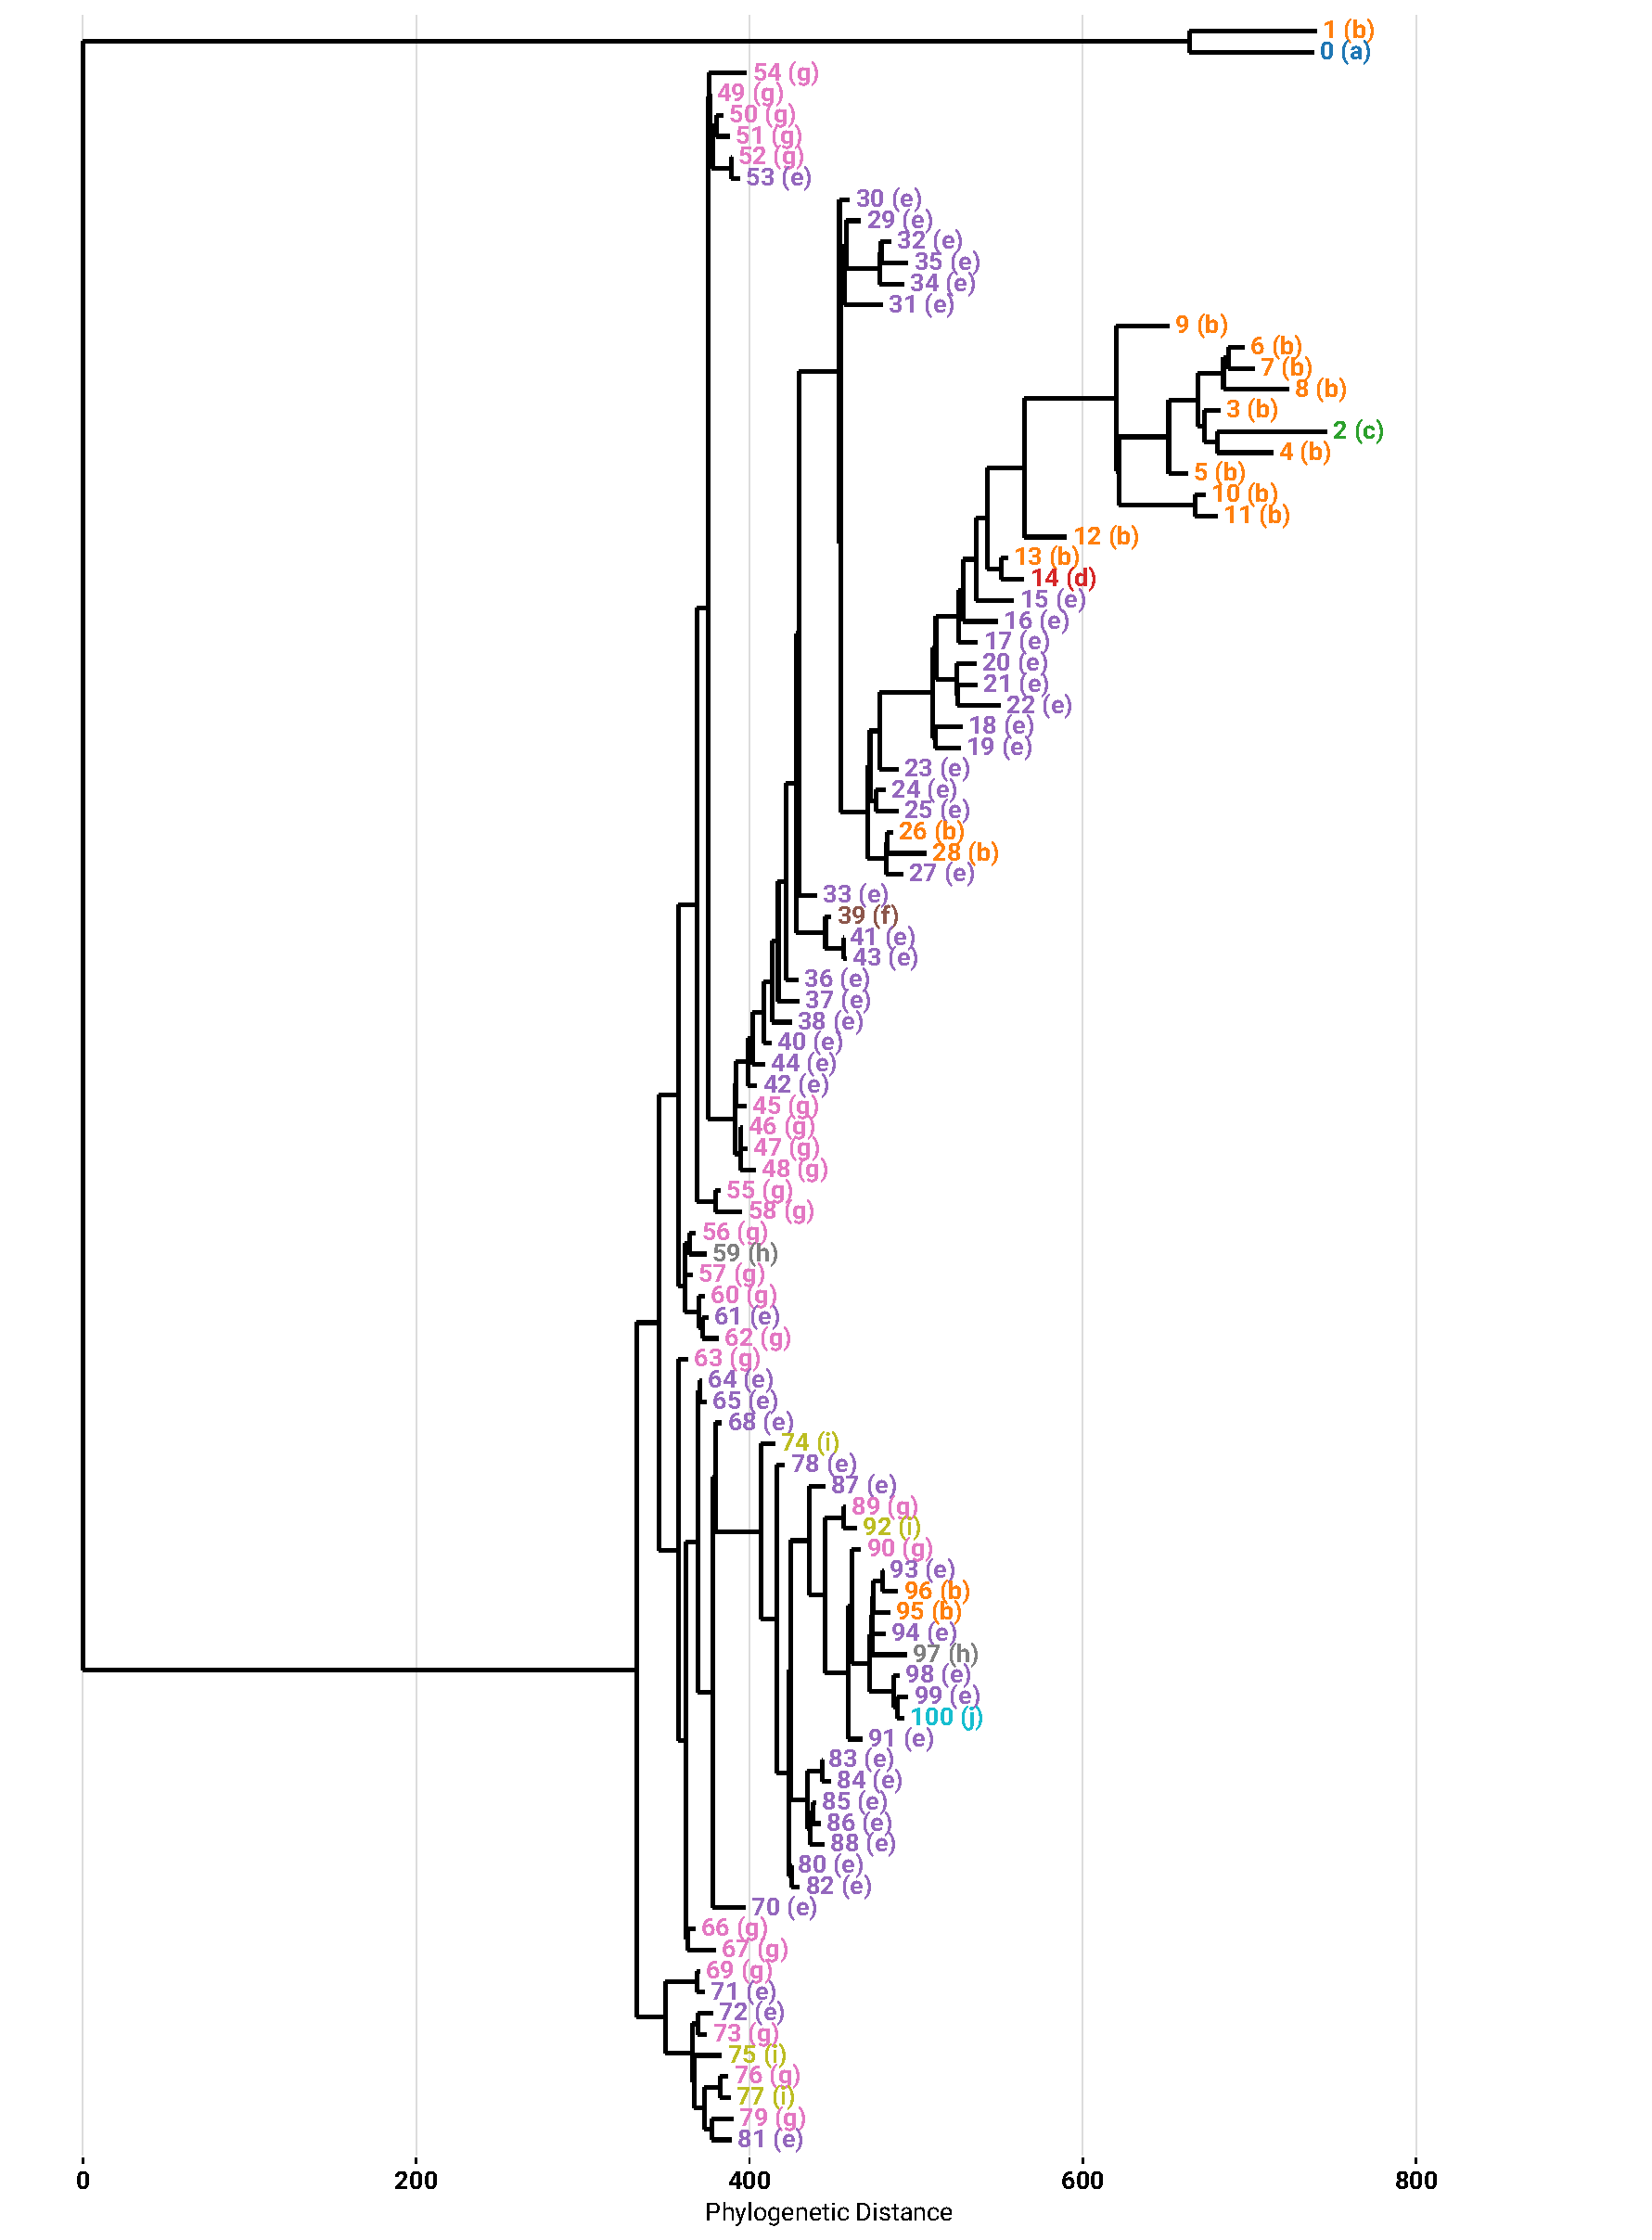
\includegraphics[width=0.8\linewidth]{{submodule/dishtiny_event_tag_phylogenetics/teeplots/phylo_tree_no_outliers/viz=draw+ext=}}

\caption{
Phylogeny of sampled focal strain representatives across stints reconstructed using neighbor-joining algorithm \citep{cock2009biopython}.
Each leaf node corresponds to a sampled representative.
Representatives from stints 0 and 1, which share no common ancestry with representatives from other stints, are excluded.
Numbers refer to stint that each representative was sampled from.
Color coding and parentheticals of stint labels correspond to qualitative morph codes described in Table \ref{tab:morph_descriptions}.
}
\label{fig:phylo_nj_tree}
\end{figure*}
